\documentclass[usenames,dvipsnames]{beamer}
\usetheme{Berlin}
\usepackage[utf8]{inputenc}
\usepackage[english]{babel}
\usepackage{graphicx}
\usepackage{url}
\usepackage{multicol}
\usepackage{enumitem}
\usepackage{fancyvrb}

\graphicspath{ {images/} }

\title{CodeQL U-Boot challenge}
\subtitle{}
\author{Alexander Livenets \\ Alberto Mardegan}
\institute{}
\date{12 May 2020}

\newcommand{\codeinline}[1] {\texttt{\smaller[2]{#1}}}
\newcommand{\greenalert}[1] {\alert{\textcolor{green}{#1}}}
\newcommand{\bluealert}[1] {\alert{\textcolor{blue}{#1}}}
\newcommand{\redalert}[1] {\alert{\textcolor{red}{#1}}}
\begin{document}

\AtBeginSection[]
{
\begin{frame}
\frametitle{Table of Contents}
\tableofcontents[currentsection]
\end{frame}
}

\setbeamertemplate{endpage}{%
\begin{frame}
\center \Huge Thanks!
\end{frame}
}

\begin{frame}
\titlepage
\end{frame}

\section{CodeQL}
\begin{frame}
\frametitle{CodeQL}
CodeQL is a powerful query language that allows to analyze code
to see data flows and vulnerabilities
\end{frame}

\begin{frame}
\centering
\huge CodeQL $\thicksim$ SQL for the code
\end{frame}

\section{Examples}
\begin{frame}[fragile]
\frametitle{\secname}
\small
\begin{verbatim}
from /* variable declarations... */
where /* logical formulas... */
select /* expressions... */
\end{verbatim}
\end{frame}

\begin{frame}[fragile]
\frametitle{\secname}
\small
\begin{verbatim}
from int x, int y
where x = 6 and y = 7
select x * y
\end{verbatim}
\end{frame}

\begin{frame}[fragile]
\frametitle{\secname}
\small
\begin{verbatim}
class SmallInt extends int {
  SmallInt() { this in [1..10] }
  int square() { result = this*this }
}

from SmallInt x, SmallInt y, SmallInt z
where x.square() + y.square() = z.square()
select x, y, z
\end{verbatim}
\end{frame}

\section{CodeQL for C/C++}
\begin{frame}[fragile]
\frametitle{\secname}
\small
\begin{verbatim}
import cpp

from IfStmt ifstmt, Block block
where ifstmt.getThen() = block
  and block.getNumStmt() = 0
select ifstmt, "This 'if' statement is redundant."
\end{verbatim}
\end{frame}

\begin{frame}
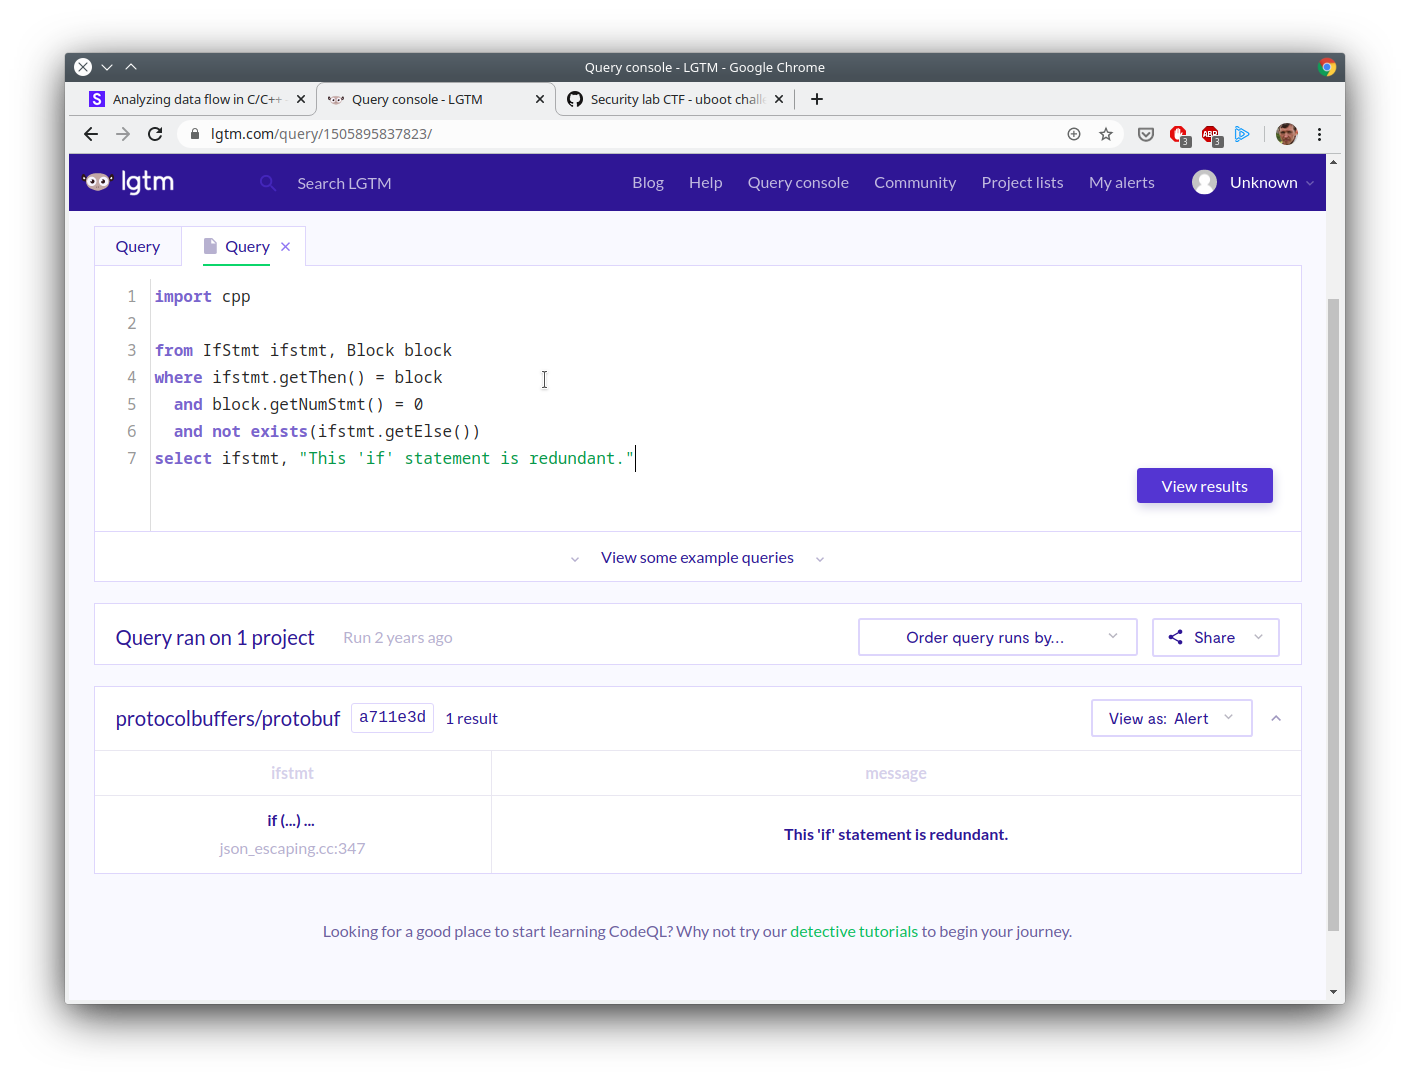
\includegraphics[scale=0.25]{codeql-example-1.png}
\end{frame}

\begin{frame}[fragile]
\frametitle{\secname}
\small
\begin{semiverbatim}
import cpp		                  \bluealert{/* Use C++ language package */}

from IfStmt ifstmt, Block block \bluealert{/* select all ifs */}
where ifstmt.getThen() = block
  and block.getNumStmt() = 0    \bluealert{/* that have empty then block */}
  not ifstmt.hasElse()		      \bluealert{/* and don't have else block */}
select ifstmt, "This 'if' statement is redundant."
\end{semiverbatim}
\end{frame}

\section{U-Boot Challenge}
\begin{frame}
\frametitle{\secname}
Task: find known RCE (Remote Code Execution) vulnerabilities in U-Boot using CodeQL.

Hints: they all based on \texttt{memcpy} and reading size from network, also using \texttt{ntoh*} function family.
\end{frame}

\begin{frame}[fragile]
\frametitle{Task 0}
  Find the definition of \texttt{memcpy} and \texttt{ntoh*}
  \footnotesize
  \begin{columns}
    \begin{column}{0.5\textwidth}
      \begin{verbatim}
import cpp

from Function f
where f.getName() = "memcpy"
select f
      \end{verbatim}
    \end{column}
    \begin{column}{0.5\textwidth}
      \begin{verbatim}
import cpp

from Macro m
where m.getName() = "ntohl" or 
  m.getName() = "ntohll" or
  m.getName() = "ntohs"
select m
      \end{verbatim}
    \end{column}
  \end{columns}

\end{frame}

\begin{frame}[fragile]
\frametitle{Task 1}
  Find the calls of \texttt{memcpy} and \texttt{ntoh*}
  \footnotesize
  \begin{columns}
    \begin{column}{0.5\textwidth}
      \begin{semiverbatim}
import cpp

from FunctionCall fc
where fc.\bluealert{getTarget()}
  .getName() = "memcpy"
select fc
      \end{semiverbatim}
    \end{column}
    \begin{column}{0.5\textwidth}
      \begin{semiverbatim}
import cpp

from Macro m
where m.getName() = "ntohl" or 
  m.getName() = "ntohll" or
  m.getName() = "ntohs" 
select m\bluealert{.getAnInvocation()}  
      \end{semiverbatim}
    \end{column}
  \end{columns}
\end{frame}

\begin{frame}[fragile]
\frametitle{Task 2}
Find all top level expressions for macro invocations
\footnotesize
\begin{semiverbatim}
import cpp

class NtohsMacroInvocation extends Expr \{
  NtohsMacroInvocation() \{ 
      \bluealert{exists(Macro m | m.getName() = "ntohs"  or}
      \bluealert{  m.getName() = "ntohll" or}
      \bluealert{    m.getName() = "ntohl"}
      \bluealert{  | this = m.getAnInvocation().getExpr())}
    \}
\}

from NtohsMacroInvocation mi
select mi
\end{semiverbatim}
\end{frame}

\begin{frame}[fragile]
\frametitle{Taint Tracking}
\textbf{\textit{tainted function call}} - the function call that gets unsanitized data as input.
\\
\begin{semiverbatim}
int pkt_size = read_packet_size_from_network(); 
char *pkt = (char*)malloc(pkt_size); \redalert{// TAINTED!!!}
\end{semiverbatim}
\end{frame}

\begin{frame}[fragile]
\frametitle{Resulting code}
Resulting solution (9 of 13 CVEs)
\tiny
\begin{semiverbatim}
import cpp
import semmle.code.cpp.dataflow.TaintTracking
import DataFlow::PathGraph
\end{semiverbatim}
\begin{columns}
\begin{column}{0.5\textwidth}
\begin{semiverbatim}
class NtohsMacroInvocation extends Expr \{
  NtohsMacroInvocation() \{ 
      \bluealert{exists(Macro m | m.getName() = "ntohs"  or}
      \bluealert{  m.getName() = "ntohll" or}
      \bluealert{    m.getName() = "ntohl"}
      \bluealert{  | this = m.getAnInvocation().getExpr())  }
  \}
\end{semiverbatim}
\end{column}
\begin{column}{0.5\textwidth}
\begin{semiverbatim}
class Config extends TaintTracking::Configuration \{
  Config() \{ this = "NetworkToMemFuncLength" \}
  override predicate isSource(DataFlow::Node source) \{
    \bluealert{source.asExpr() instanceof NtohsMacroInvocation}
  \}
  override predicate isSink(DataFlow::Node sink) \{
    \bluealert{exists (FunctionCall fc |}
    \bluealert{  sink.asExpr() = fc.getArgument(2) and}
    \bluealert{  fc.getTarget().getName() = "memcpy"}
    \bluealert{)}
  \}
\}
\end{semiverbatim}
\end{column}
\end{columns}
\begin{semiverbatim}
from Config cfg, DataFlow::PathNode source, DataFlow::PathNode sink
where cfg.hasFlowPath(source, sink)
select sink, source, sink, "ntoh flows to memcpy"
\end{semiverbatim}
\end{frame}

\section{References}
\begin{frame}
\frametitle{\secname}
\footnotesize
\begin{itemize}[leftmargin=*]
  \item \url{https://help.semmle.com/QL/learn-ql/introduction-to-ql.html}
  \item \url{https://securitylab.github.com/ctf/uboot}
  \item \url{https://github.com/alivenets/codeql-u-boot-challenge}
\end{itemize}
\end{frame}

\usebeamertemplate{endpage}

\end{document}
